
% スタイルファイルの指定
% パッケージを使用する場合,ここで全て指定する.
\documentstyle[cite,a4j,twoside,12pt,enumerate,graphicx,listings,amssymb,subcaption,amsmath]{jbmdthesis}

% ヘッダを追加する
\pagestyle{headings}

% 画像元のパスの追加
\graphicspath{{figure/}}

\begin{document}

% 図,表,節などを参照するためのコマンドを定義
% これらのコマンドの使い方は template/ 内の Readme.md を参照すること
\newcommand{\fig}[1]{{図~\ref{fig:#1}}}
\newcommand{\subfig}[2]{{図~\ref{fig:#1}}~{(\subref{fig:#2})}}
\newcommand{\tab}[1]{{表~\ref{tab:#1}}}
\newcommand{\refchap}[1]{第{\ref{sec:#1}~章}}
\newcommand{\refsec}[1]{{\ref{sec:#1}~節}}

% ページ番号をアラビア数字にする(0,1,2,..)
\pagenumbering{roman}


% ---------- ユーザ入力ここから ----------
% タイトルページの情報
\title{\bf 容量効率を意識したソース・タグ値に基づくセグメント化による \\
発行キューの電力削減}
\author{\bf 森 健一郎}
\date{3} % 令和~年

% 表紙を出力(自分の所属に応じてコメントを外す)
\minfotitle   % 修論
% \belectitle   % 卒論
% ---------- ユーザ入力ここまで ----------



% 概要を出力
{ 
  % 目次に影響がでないように, 
  % setlength のスコープを abstract 内だけに限定するためのブロック

  % 行間の調整
  \setlength{\baselineskip}{2.2em}
  
\chapter*{概要}
\markboth{概要}{概要}
近年のサーバー・アプリケーションや,JavaScriptで書かれたWebアプリケーションでは,従来のアプリケーションと比べて命令キャッシュ・ミスが特に多く発生することが知られている.これに対し,命令キャッシュ向けのプリフェッチャが多く研究されており,非常に高いキャッシュ・ヒット率が達成されている.しかし,それらのプリフェッチャでは高い性能をもつものほど大きな追加資源が必要になる.例えば,最先端の命令プリフェッチャであるProactive Instruction Fetchでは,L1命令キャッシュそのものより大きなテーブルを必要とする.また,プリフェッチのミスに対するカバー率こそ高いものの,無駄なプリフェッチを多く実行してしまい,電力を無駄に消費してしまう場合がある.

これに対し,本論文では命令プリフェッチのアプローチではなく,フェッチ・ステージのパイプライン構造の工夫によりフェッチ・スループットを向上させる手法を提案する.本提案手法はプリフェッチャと異なり,複雑な機構や大きなテーブルも必要なく,無駄なメモリアクセスを全く行わない.さらに,性能低下のデメリットなしに命令キャッシュ・ミスによるストールを削減し,フェッチ・スループットを向上させることができる.
提案手法をサーバー向けのベンチマークを用いて評価したところ,プリフェッチを行わない場合と比較して最大 25.8\%,平均で13.0\%の性能向上を達成した.また,最先端の命令プリフェッチャと比較して平均4.8\%の性能向上が得られることを確認した.

}

% 目次を出力
\tableofcontents

% ページ番号のリセット
\clearpage 
\pagenumbering{arabic}

% 行間の調整(これ以降ずっとこの行間)
\setlength{\baselineskip}{2.2em}



% ---------- ユーザ入力ここから ----------
% 各章の記述

\chapter{はじめに}
\label{sec:introduction}
近年のプロセッサは,命令キャッシュ・ミスによる性能低下が問題となっている.これは,現代のアプリケーションの命令ワーキング・セットが大きくなっていることに由来する.このようなアプリケーションの例として,オンライントランザクション処理などのサーバー向けのアプリケーション~\cite{Ranganathan1998,Vaidya2008,Ferdman2012}や,JavaScriptを用いたWebアプリケーション~\cite{Zhu2015,Chadha2014},クラウドのアプリケーション~\cite{Ferdman2012,Ayers2019}がある.これらのアプリケーションは,命令フットプリントが膨大であり,L1命令キャッシュに収まらないため,命令キャッシュ・ミスが多く発生する.命令キャッシュ・ミスが発生すると,プロセッサに実行できる命令を供給できなくなるため,それにより性能が低下する.これは近年の高性能なアウト・オブ・オーダー実行方式のプロセッサにおいても命令キャッシュ・ミスにおけるストールは隠蔽することが難しいため,重要な問題である.

この問題に対し,命令キャッシュ・ミスを減らす手法として,命令プリフェッチャがある.命令プリフェッチャは,ある命令が要求される前に,その要求を先読みして下位レベルのメモリへアクセスを行い,あらかじめその命令をキャッシュへと転送する.これを命令プリフェッチという.命令プリフェッチが成功すると,命令キャッシュ・ミスを回避できるため,性能低下を抑えることができる.

命令プリフェッチャには様々なものが提案されている.例えば,単純なものとしてミスしたラインの次のラインをプリフェッチするネクストライン・プリフェッチャがある.また,分岐予測器が持つ情報を使用するFetch Directed Instruction Prefetching~\cite{Reinman1999}や,命令キャッシュ・ミスのストリームを記録して命令プリフェッチを行うTemporal Instruction Fetch Streaming~\cite{Ferdman2008},及びそれを改良した非常に高いプリフェッチ効果をもつProactive Instruction Fetch (PIF)~\cite{Ferdman2011}などが提案されている.

しかし,これらのプリフェッチャは,性能が高いものほど非常に大きなコストが必要になる.なぜなら,有効なプリフェッチを行うためには,複雑なキャッシュ・ミス・パターンを予測するアルゴリズムをハードウェアで実現する必要があるからである.特にPIFは,命令キャッシュ・ミスを90\%以上削減することが可能であるが,必要なストレージのサイズは一般的なL1命令キャッシュよりも非常に大きい(L1命令キャッシュが32KBに対し,200KB程度).さらに,このようなプリフェッチャは,プリフェッチのミスに対するカバー率こそ高いものの,無駄なプリフェッチを実行することもあり,その分電力を余分に消費してしまう.

そこで,本論文では命令プリフェッチのアプローチではなく,命令フェッチ部のパイプライン構造を工夫することによって命令フェッチのスループットを向上させる以下のような手法を提案する.
\begin{enumerate}
  \item 従来の命令フェッチ・パイプラインでは,L1命令キャッシュがヒットすることを前提としてパイプラインが設計されており,命令がフェッチされるとその命令は直ちに次のステージが送られる.これに対し,本研究ではMiss-assuming Pipeline (MAP) と呼ばれる新しいパイプライン構造を提案する.MAP は L1 命令キャッシュのミスを前提としてパイプラインが設計されており,命令キャッシュがヒットしてもミスしても常に一定のレイテンシでフェッチを行う.この動作により,MAP では命令キャッシュ・ミスが発生してもフェッチのスループットを損なうことなく,実行を継続できる.
  \item しかし,MAP は従来のパイプラインと比べてパイプライン段数が増加なるため,分岐予測ミス・ペナルティが増加してしまう.MAPの 利点を最大限活用しつつこの欠点に対処するために,本研究ではフェッチのパイプライン構造を,従来のパイプラインと MAP の間で動的に切り替えて使用するアーキテクチャを提案する.同時に,本論文ではこのアーキテクチャによって得られる恩恵を最大化するための最適なパイプラインの切り替えアルゴリズムを提案する.このアルゴリズムを用いると,MAP による分岐予測ミス・ペナルティ増加の影響を最小にすることができ,得られる恩恵を最大化することができる.
\end{enumerate}

提案手法は,プリフェッチャとは異なり無駄なメモリ・アクセスを全く行わない.また,従来のプリフェッチャのような複雑な機構や大きなテーブルも必要なく,非常に低コストで構成することができる.さらに,本提案手法を適用すると,性能低下のデメリットなしに命令キャッシュ・ミスによるストールを削減でき,命令キャッシュ・ミスが多く発生するような状況においては,大きな性能向上が期待できる.

本論文の構成は次の通りである.まず,\refchap{related_work}で関連研究を示す.\refchap{miss_assumed_pipeline}では MAP について説明する.その後,\refchap{hybrid_arc}で従来の構成と MAP を組み合わせたアーキテクチャについて述べ,\refchap{sw_algorithm}では提案するパイプラインの切り替えアルゴリズムについて述べる.\refchap{evaluation}では提案手法の評価を行い,最後に\refchap{summary}でまとめる.



\chapter{Miss-assuming Pipeline (MAP)}
\label{sec:miss_assumed_pipeline}
本章では,提案手法の一つであるMAPについて説明する.まず,\refsec{map_abstract}でMAPの概要を述べた後,\refsec{map_structure}でMAPの構造を示す.その後,\refsec{map_different}で MAP の動作を従来のパイプラインと比較しながら示し,\refsec{tradeoff}で従来のパイプラインに対するトレードオフについて述べる.

\section{概要}
\label{sec:map_abstract}

本研究では,命令キャッシュ・ミスによる性能低下を抑制するために,Miss-assuming Pipeline (MAP)という新しい命令フェッチのパイプライン構造を提案する.従来のプロセッサは,命令キャッシュ・アクセス時に,キャッシュがヒットすることを前提としてパイプラインが設計されている.これに対し,MAP は命令キャッシュ・アクセス時にキャッシュ・ミスが発生することを前提としてパイプラインが設計されている.このことを\fig{pipeline}を用いて説明する.同図はプロセッサのパイプライン・ステージを図示したものであり,L1, L2,ID,EX, WB はそれぞれ L1 キャッシュ・アクセス,L2 キャッシュ・アクセス,デコード,実行,ライトバック・ステージを表しており,NOP は何もしない(no-operation)で命令を次のステージに渡すステージを表している.なお,説明を簡単にするために,本論文の説明では L1 キャッシュのレイテンシを 1 サイクル,L2 キャッシュのレイテンシを 2 サイクルと仮定する.また,L2 キャッシュは必ずキャッシュ・ヒットすると仮定する.

まず,従来のパイプラインの動作について説明する.従来のパイプラインでは,命令キャッシュがヒットした場合,\subfig{pipeline}{hap_pipeline}の上側に示すように命令が得られると即座にその命令をデコード・ステージへ送る.一方,命令キャッシュがミスした場合は,L2 キャッシュへのアクセスが必要になるため,\subfig{pipeline}{hap_pipeline}の下側に示すように L1 キャッシュ・アクセス後に 2 サイクルかけて L2 キャッシュ・アクセスを行い,得られた命令をデコード・ステージへ送る.

これに対し,MAP では,命令キャッシュがヒットした場合でも,得られた命令を即座にデコード・ステージへ送らず,L2 キャッシュのレイテンシと同じ数の NOP ステージを経由してから命令をデコード・ステージへ送る.これは,命令キャッシュがヒットしてもミスしても,命令をデコード・ステージに送るタイミングを同じにするためである.詳細は\refsec{map_different}で述べるが,この動作により MAP は命令キャッシュ・ミスが発生してもパイプラインの乱れが生じず,性能が低下しないという特徴を持つ.命令キャッシュがミスした場合の動作は,従来のパイプラインと同じである.

なお,命令キャッシュのミスを前提としている MAP に対し,従来のパイプラインは命令キャッシュのヒットを前提としているため,本論文では以降,従来のパイプラインのことを MAP と対比して Hit-assuming Pipeline (HAP) と呼ぶ.

% 図を使う例: figure 環境を使用

% \begin{figure}[tb]
%   \centering
%   \includegraphics[scale=.5]{hoge.eps}
%   \caption{例1}
%   \label{fig:hoge}
% \end{figure}



% 副図を使う例: minipage と subcaption を使用

% \begin{figure}[tb]
%   \begin{minipage}[htb]{1\hsize}
%     \centering 
%     \includegraphics[keepaspectratio, scale=0.8]{hap_pipeline.eps}
%     \vspace{.3cm} % <-- vspace で縦方向の位置を調節できる
%     \subcaption{従来のパイプライン (HAP: Hit-Assuming Pipeline)}
%     \label{fig:hap_pipeline}
%   \end{minipage}
%   \begin{minipage}[htb]{.97\hsize}
%     \vspace{1.3cm}
%     \centering
%     \includegraphics[keepaspectratio, scale=0.8]{map_pipeline.eps}
%     \vspace{.3cm}
%     \subcaption{MAP: Miss-Assuming Pipeline}
%     \label{fig:map_pipeline}
%   \end{minipage}
%   \vspace{.8cm}
%   \caption{各パイプラインの命令処理工程}
%   \label{fig:pipeline}
% \end{figure}




% 
\chapter{関連研究}
\label{sec:related_work}
本章では,IQ に関連する研究について述べる.\refsec{relate_IQ}で IQ に関する一般的な関連研究に関して説明し,\refsec{relate_IQ} で IQ の研究のうち,電力に関係する研究を述べる.

\section{IQ に関する関連研究}
\label{sec:relate_IQ}
Palacharlaらは,命令発行幅とIQのサイズを変化させた時の,ウェイクアップ論理と選択論理の遅延を評価した~\cite{Palacharla1997}.また,遅延を小さくするために,IQを複数のFIFOバッファで構成し,依存する命令を同じFIFOバッファに割り当てる依存ベースのIQを提案した.この手法では,各バッファの先頭の命令のみ発行可能かチェックすれば良いので,回路が単純化され遅延が減少する.

Starkらは,IPCをほとんど低下させずに,ウェイクアップ論理と選択論理をパイ
プライン化する手法を提案した\cite{Stark2000}.この手法では,投機的にウェイクアップを行うことで,依存する命令を連続するサイクルで発行できるようにした.

五島らは,ウェイクアップ論理を従来のCAMではなく,依存行列と呼ぶRAMで構成する手法を提案した\cite{goshima2001}.これによって比較器を用いずに依存する命令をウェイクアップすることが可能で,ウェイクアップの遅延を短縮できる.

Sassoneらは,依存行列の遅延と電力をより小さくするための手法を提案した\cite{sassone2007}.具体的には,従来はすべての命令について,その古さを完全に追跡していたのに対して,命令をグループ化してグループ単位で古いものを選択する.これにより,性能低下を最小限に抑えながら,回路の規模を小さくできる.

Lebeckらは.キャッシュ・ミスするロードのような長いレイテンシの命令に依存する命令を,IQとは別の待機用バッファに入れ,その長いレイテンシの処理が完了するまでIQに挿入しないという方式を提案した\cite{Lebeck2002}.これによって,IQが待機する命令で埋ることによって起こるストールの頻度が減り,性能が向上する.

Raaschらは,IQをいくつかのセグメントに分割する方式を提案した\cite{Raasch2002}.この方式では,各命令の依存命令チェーンのレイテンシを元に割り当てるセグメントが決定される.そして,発行可能になる直前に最下位セグメントである発行バッファに命令を移動する.この発行バッファでのみ発行を行うことで,すべてのエントリから発行できる通常のIQと比較して遅延を短縮できる.

Kimらは,レイテンシが互いに1サイクルの依存関係のある2つの命令をグループ化し,1つの命令としてIQのエントリでスケジューリングすることで,依存グラフのエッジのレイテンシ短縮とキューの容量効率を上げる手法を提案した\cite{Kim2003}.

Gibsonらは,依存する命令をポインタでつなぎ,ポインタをたどることでウェイクアップを行う手法を提案した\cite{Gibson2010}.この方式によりCAMが不要になり,電力を削減できる.

安藤らは,実行プログラムの命令レベル並列性(ILP)とメモリ・レベル並列性(MLP)に応じて IQ の方式を切り替える手法を実装した\cite{Ando2019}.ILP と MLP のいずれかが高い場合は IQ の容量効率が重要であるため,ランダム・キューで実行する.ILP も MLP もいずれも低い場合には,容量効率よりも正しい発行優先度のほうが重要であるためサーキュラー・キューで実行する.

甲良らは,実行プログラムの ILP と MLP に応じて IQ のサイズを変化させる手法を提案した\cite{Kora2013}.本手法では,いずれかが高い場合には,IQ の容量が重要となるため IQ のエントリ数を増加し,どちらも低い場合には IQ のエントリ数を減少させる.

\section{IQ の電力削減に関する関連研究}
\label{sec:relate_energy}
Folegnaniらは,空のエントリの比較器や既にレディなオペランドを持つ比較器など,タグを比較する必要がない比較器を動作させないことで,消費エネルギーを削減する手法を提案した\cite{folegnani2001}.

Ponomarev らは,リソース要求に応じて 発行キューのサイズをリサイズすることにより,消費エネルギーを削減する手法を提案した~\cite{ponomarev2001} .

Ernstらは,IQに入ってくる命令のうちのほとんどが,はじめから少なくとも1つのソース・オペランドがレディであると指摘した\cite{ernst2002}.そしてIQに,2つのソース・オペランドを保持できるエントリに加えて,1つのソース・オペランドのみ保持できるエントリと,ソース・オペランドを保持しないエントリを用意し,レディでないソース・オペランドの数に応じていずれかにディスパッチする手法を提案した.さらにこの手法を実現するために,命令の2つのオペランドの内,あとにレディになるオペランドを予測する手法である Last Tag Prediction も提案した.

Sembrant らは,クリティカル・パス上にない命令を発行キューとは別のバッファに入れ,ディスパッチを遅延させることによって,性能を低下させずに発行キューのサイズを小さくする手法を提案した~\cite{Sembrant2015}.

Homayoun らは,キャッシュ・ミスの処理中に発行幅を半減させることで,IQの消費電力を削減する手法を提案した\cite{H.Homayoun2011}.発行幅半減中に元の発行幅の半分以上の命令が発行される場合,一時的にその命令を小さなバッファに移動させることで対応している.

松田らはウェイクアップ時のタグ比較を 2 段階に分割することによりエネルギー削減を行う方法を提案した\cite{kobayashi-thesis, matsuda-thesis}.この方法では,タグの比較を高位ビットと低位ビットに分割し,低位ビットの比較を最初のサイクルで行う.そして低ビットが一致していた場合のみ,次のサイクルで高位ビットの比較を行うことによってエネルギーを削減する.また,タグの 2 段階比較には,ウェイクアップに 2 サイクル必要であるため性能が低下するという欠点が存在する.これに対し本手法では,クリティカルパス上にある命令のみ 1 サイクルで比較を行い性能低下の軽減を行う.



\chapter{まとめ}
\label{sec:summary}
LSIの微細化の進展に伴って,経年劣化が加速し摩耗故障が増加する問題が深刻になっている.この故障は,デバイスの温度に関して指数関数的に加速するため,チップ内のホット・スポットの解消が求められている.

発行キューはこのホット・スポットの 1 つとして知られている.この主な原因はウェイクアップ時の多数のタグ比較である.本論文では,ウェイクアップ時のタグ比較回数を削減するために,発行キューをセグメント化する方法を提案した.また,提案手法におけるタグ比較削減の効果を高める手法であるスワップとサブ・セグメント及び,提案手法によって生じる性能低下を抑制する手法である SWITCH 方式を合わせて提案した.

提案手法を SPEC CPU 2017 を使って評価したところ,性能低下を最大でも 5\% 以下に抑えつつ,タグ比較回数を 82\% 削減できることを確認した.



% 付録(必要に応じてコメントを外したり,新たに追加する)
% \appendix
% 
\chapter{提案手法のその他の工夫}
\label{sec:appendix1}
提案手法によるタグ比較回数をより減らすための工夫として,Last Tag Prediction(LTP) という手法が有効ではないかと考え,シミュレータに実装し評価を行った.本章では,LTP とその評価結果に関して説明する.なお,評価の結果,LTP はあまり効果がないことがわかったため,最終的な提案手法には実装していない.

\section{LTP:Last Tag Prediction}
CONSARVARTIVE 方式 において,第 1 ソース・タグと第 2 ソース・タグがどちらもレディでない命令は,以下のアルゴリズムでセグメントを選択すると述べた.

\begin{itemize}
  \item サブ・セグメントを使用しない場合:第 1 ソース・タグでセグメントを選択する.選択したセグメントに空きがない場合,スワップして第 2 ソース・タグをもとにセグメントを決定する.なおも空きがない場合はストールする.
  \item サブ・セグメントを使用する場合:第 1 ソース・タグでメイン・セグメントを,第 2 ソース・タグでサブ・セグメントを選択する.選択したセグメントに空きがない場合,スワップを行い,第 2 ソース・タグでメイン・セグメントを,第 1 ソース・タグでサブ・セグメントを選択する.スワップしてなおも空きがない場合はストールする.
\end{itemize}

このアルゴリズムにおいて,スワップする場合としない場合に選択されるセグメントのどちらにも空きがある場合を考える.このような場合,CONSERVATIVE のアルゴリズムでは,スワップを行わずにディスパッチするセグメントを決定する.

このような場合に,レディとなるのがより遅く,比較がより多く行われるソース・オペランドのタグ(ラスト・タグ)を第 1 ソース・タグのフィールドに書き込むようにセグメントを選択すれば,タグ比較回数をより多く削減できると考えられる.ただし,ラスト・タグがどちらになるかという情報はデコード時にはわからないため,予測を行う必要がある.

ラスト・タグの予測方法は,論文~\cite{ernst2002}で提案されている.この方法を Last Tag Prediction(LTP)と呼ぶ.以下,LTP による予測とセグメントの選択方法に関して説明する.

\begin{figure}[htb]
  \centering
  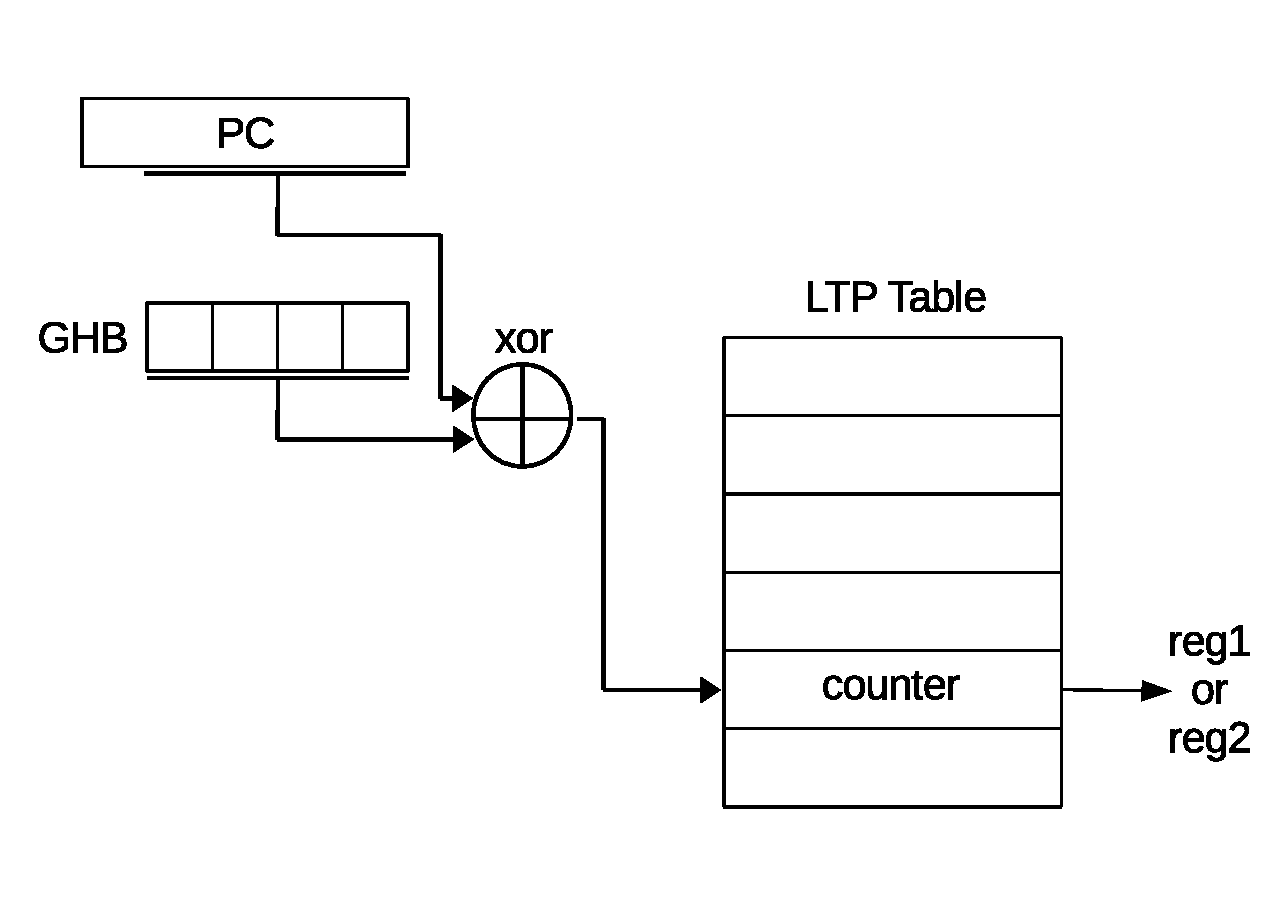
\includegraphics[keepaspectratio, scale=.8]{ltp}
  \caption{LTP の構成}
  \label{fig:ltp}
\end{figure}

LTP は,\fig{ltp}のように.命令の PC の下位ビットビットとグローバル分岐履歴(GHB:Global History Buffer)のハッシュをインデクスとするテーブル(LTP Table)で構成される.LTP Table の各エントリは 2 ビットの飽和型アップ・ダウン・カウンタで構成され,このカウンタは,値が 0 または 1 の場合に第 1 ソース・タグがラスト・タグであることを示し, 2 または 3 の場合に第 2 ソース・タグがラスト・タグであることを示す.予測と学習の方法について説明する.
  
\subsection{予測方法}
命令ディスパッチ時に,第 1 ソース・タグと第 2 ソース・タグがともにレディでなく,なおかつスワップした場合としない場合に選択されるセグメントがいずれもディスパッチ可能な場合に予測が行われる.予測の際には,PC と GHB のハッシュを用いてテーブルを検索し,該当するエントリのカウンタ値を読み出す.

第 1 ソース・タグがラスト・タグであると予測された場合には,スワップを行なわずにセグメントを選択しディスパッチする.第 2 ソース・タグがラスト・タグであると予測された場合には,スワップを行いセグメントを選択し,ディスパッチする.
  

\subsection{学習方法}
学習は命令発行時に,ディスパッチ時に予測を行った命令でのみ行われる.命令発行時に,第 1 ソース・タグと第 2 ソース・タグがレディとなったサイクルを比較する.第 1 ソース・タグ のほうが遅かった場合にはカウンタをデクリメントし,第 2 ソース・タグのほうが遅かった場合にはカウンタをインクリメントする.

\section{LTP の評価}

% 発表実績(なければコメントアウトしておく)

\chapter*{発表実績}
\addcontentsline{toc}{chapter}{発表実績}
\begin{itemize}
  \item 森健一郎, 安藤秀樹, ``容量効率を意識したソース・タグ値に基づくセグメント化による発行キューのエネルギー削減'', 情報処理学会研究報告, Vol.2020-ARC-241, No.3, pp.1-12, 2020年7月
\end{itemize}

% 謝辞

\chapter*{謝辞}
\addcontentsline{toc}{chapter}{謝辞}
本研究を進めるにあたり,多大なる御指導と御鞭撻を賜わりました名古屋大学大学院工学研究科 情報・通信工学専攻 安藤秀樹教授に心より感謝いたします.また,本研究の遂行を支えてくださいました,名古屋大学大学院工学研究科情報・通信工学専攻安藤研究室の諸氏に深く感謝します.

% ---------- ユーザ入力ここまで ----------


% 参考文献
\bibliographystyle{IEEEtran} 
\bibliography{ref}

\end{document}
